\begin{frame}
  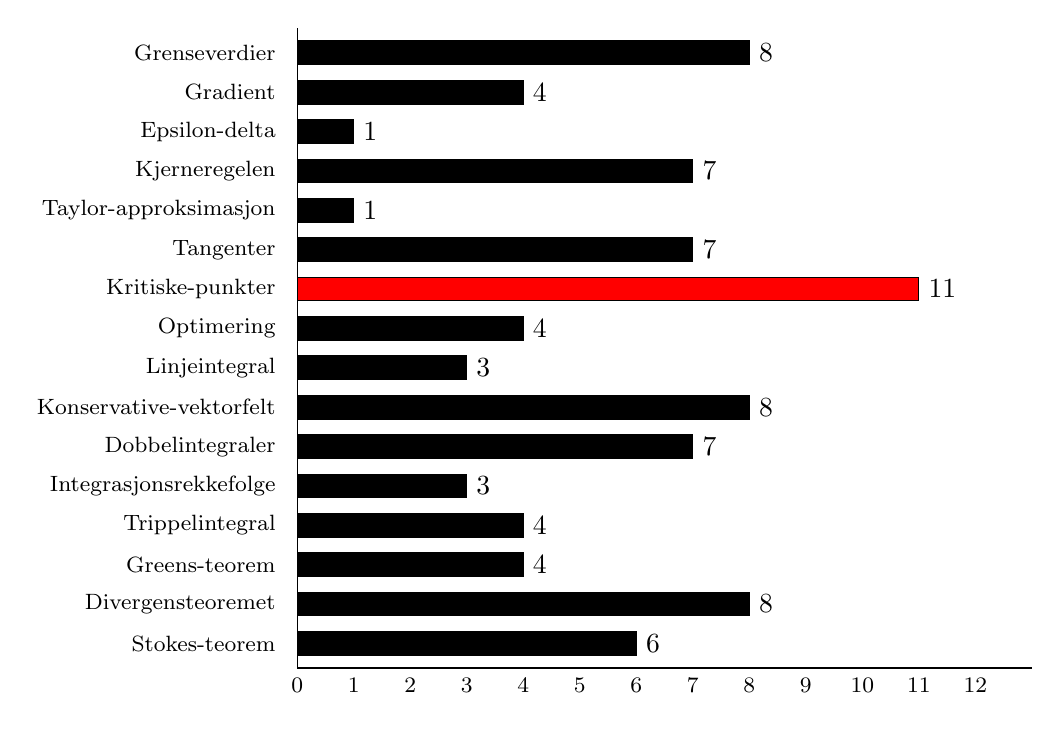
\begin{tikzpicture}
    \begin{axis}[ xbar=0pt, /pgf/bar shift=0pt, legend style={ legend columns=4,
        at={(xticklabel cs:0.5)}, anchor=north, draw=none }, ytick={0,...,15},
      ytick style={draw=none},% <- added
      axis y line*=none, axis x line*=bottom, tick label
      style={font=\footnotesize}, legend style={font=\footnotesize}, label
      style={font=\footnotesize}, xtick style={draw=none},% <- added
      xtick={0,1,...,12}, width=.9\textwidth, bar width=3mm, y dir = reverse,
      xmin=0, xmax=13, area legend,
      y=5mm, enlarge y limits={abs=0.625},
      style={text=black}, every axis plot/.append style={fill},
      nodes near coords, nodes near coords,
      yticklabels={%
        {\topicref{Grenseverdier}},
        {\topicref{Gradient}},
        {\topicref{Epsilon-delta}},
        {\topicref{Kjerneregelen}},
        {\topicref{Taylor-approksimasjon}},
        {\topicref{Tangenter}},
        {\topicref{Kritiske-punkter}},
        {\topicref{Optimering}},
        {\topicref{Linjeintegral}},
        {\topicref{Konservative-vektorfelt}},
        {\topicref{Dobbelintegraler}},
        {\topicref{Integrasjonsrekkefolge}},
        {\topicref{Trippelintegral}},
        {\topicref{Greens-teorem}},
        {\topicref{Divergensteoremet}},
        {\topicref{Stokes-teorem}}}]
      \addplot[fill=black] coordinates {(8,0)};
      \addplot[fill=black] coordinates {(4,1)};
      \addplot[fill=black] coordinates {(1,2)};
      \addplot[fill=black] coordinates {(7,3)};
      \addplot[fill=black] coordinates {(1,4)};
      \addplot[fill=black] coordinates {(7,5)};
      \addplot[fill=red] coordinates {(11,6)};
      \addplot[fill=black] coordinates {(4,7)};
      \addplot[fill=black] coordinates {(3,8)};
      \addplot[fill=black] coordinates {(8,9)};
      \addplot[fill=black] coordinates {(7,10)};
      \addplot[fill=black] coordinates {(3,11)};
      \addplot[fill=black] coordinates {(4,12)};
      \addplot[fill=black] coordinates {(4,13)};
      \addplot[fill=black] coordinates {(8,14)}; 
      \addplot[fill=black] coordinates {(6,15)};
    \end{axis}
  \end{tikzpicture}
\end{frame}

\begin{frame}
  \subsection{Kritiske punkter}\label{subsec:Kritiske-punkter}
  \only<1>{\frametitle{Kritiske punkter}}
  \begin{theorem}[Annenderivertetesten i to variable]
    La $\A$ være et punkt kritisk punkt ($\nabla f(\A) = 0$) for en funksjon
    $f(x,y)$ med kontinuerlige annenordens partiellderiverte. Definer $D(x,y)$
    som
    %
    \begin{equation*}
      D(x,y) :=
      \begin{vmatrix}
        f_{xx} & f_{xy} \\ f_{yx} & f_{yy}
      \end{vmatrix}
      = \underbrace{f_{xx}}_{A}\underbrace{f_{yy}}_{B} - \underbrace{(f_{xy})^2}_{C}
    \end{equation*}
    %
    \vspace{-0.75cm}
    \begin{enumerate}
      \item Hvis $D < 0$, så er $\A$ et saddelpunkt.
      \item Hvis $D > 0$ og $f_{xx}>0$, så er $\A$ et lokalt minimum.
      \item Hvis $D > 0$ og $f_{xx}<0$, så er $\A$ et lokalt maksimum.
    \end{enumerate}
    %
    Hvis $D = 0$ gir testen ingen konklusjon.
  \end{theorem}
  \visible<2->{
  \begin{intuisjon}
    \only<2>{Anta $f_{xx}f_{yy}<0$. Enten $f_{xx}<0$ og $f_{yy}>0$ eller
    $f_{yy}<0$ og $f_{xx}>0$ uansett så har funksjonen positiv krumning $\cup$ i
    den ene retningen og negativ krumning 
    i den andre $\cap$ $\Rightarrow$ åpenbart saddelpunkt (pringles).}
  \only<3>{Anta $f_{xx}f_{yy}>0$. Hvis $f_{xx}>0$ og $f_{yy}>0$ så har $f$
    positiv krumning $\cup$ omkring
    $\A$ $\Rightarrow$ minimum. (bolle) Hvis $f_{xx}<0$ og $f_{yy}<0$ så har $f$
    negativ krumning $\cap$ omkring $A$
omkring $\A$ $\Rightarrow$ maksimum. (øvre halvkule)}
\only<4>{Tilfellet $f_{xx}f_{yy} = 0$ behandles av leddet $f_{xy}^2$. Ligner funksjonen $f$ mer
på en (pringles) eller en (bolle/øvre halvkule)?}
  \end{intuisjon}}
\end{frame}

\begin{frame}
  \begin{oppgave}{K2015, Oppgave 4a}
    Funksjonen $f \colon \R^2 \to \R$ er gitt ved $f(x,y) = 2x^2 - x^4 + y^2$. Finn alle kritiske
    punkter til $f$, og avgjør om disse er lokale maksima, minima eller
    saddelpunkter. 
  \end{oppgave}%
  %
  \vspace{-0.5cm}
\begin{equation*}
  \La(x,y) := f(x,y) = 2x^2 - x^4 + y^2
\end{equation*}
%
\only<2->{De partiellderiverte blir
%
\begin{equation*}
  \diffp{\La}{x} = \only<2>{4x - 4x^3}\only<3->{4x(1-x^2)}
  \quad \text{og} \quad 
  \diffp{\La}{y} = 2y
\end{equation*}}
%
\only<4->{Likningsettet $\nabla \La = \vek{0}$ har løsninger $(0,0)$ og $(\pm
  1,0)$.} \visible<5->{Determinanten
  %
\begin{align*}
  D(x,y) = \only<5>{ f_{xx} f_{yy} - f_{xy}^2}
  \only<6>{ \diffp[2]{}{x}(2x^2 - x^4 + y^2) \diffp[2]{}{y}(2x^2 - x^4 + y^2) - \diffp{}{xy}(2x^2 - x^4 + y^2)}
  \only<7>{ \diffp{}{x}(4x-4x^2) \diffp{}{y}(2y) - \diffp{}{x}(2y)}
  \only<8->{ 8(1 - 3x^2)}\only<9->{\hspace{3.75cm}\\[-1cm]}
%
\only<9->{\intertext{Innsetning gir}\\[-0.8cm]
%
  D(0,0) \only<9>{= 8}\only<10->{>0}, \  f_{xx}(0,0) \only<9>{= 4}\only<10>{> 0} \ \ \text{og} \ \
  D(\pm 1, 0) \only<9>{= -16}\only<10->{<0}, \  f_{xx}(\pm 1,0) \only<9>{=-8}\only<10->{<0}}\\[-0.8cm]
\end{align*}
%
\only<9->{slik at $(0,0)$ er ett \only<10->{lokalt
    minimum}\only<9>{\underline{\phantom{lokalt minimum}}} og $(\pm 1,0)$ er \only<9>{\underline{\phantom{saddelpunkter}}}\only<10>{saddelpunkter}.}}
\end{frame}

\begin{frame}
  \begin{oppgave}{K2015, Oppgave 4b}
    Funksjonen $f \colon \R^2 \to \R$ er gitt ved $f(x,y) = 2x^2 - x^4 + y^2$.
    Finn største og minste verdi for $f$ på kurven $x^4 + y^2 = 4$.
  \end{oppgave}%
  %
  \vspace{-0.5cm}
  \begin{equation*}
    \La(x,y) := 2x^2 - x^4 + y^2 - \lambda (x^4 + y^2 - 4)
  \end{equation*}
%
  \only<2->{$f_{\text{min}} = \only<2-4>{?}\only<5->{0}$, $f_{\text{max}} =
    \only<2-7>{?}\only<8-9>{4}\only<10->{4 + \frac{1}{2}}$. De partiellderiverte blir
%
\begin{align*}
  & \diffp{\La}{x} = 4x - 4x^3 - 4\lambda x^3,
  &&\diffp{\La}{y} = \only<2>{2y - \lambda 2y}\only<3->{2y(1-\lambda)}
  \quad \text{og} \quad 
  &&\diffp{\La}{\lambda} = x^4 + y^2 - 4
%
\only<3>{\intertext{Fra $\La_y = 2y(1-\lambda)=0$ får vi at enten $y = 0$ eller
  $\lambda = 1$.}}
\visible<4->{\intertext{\underline{$\only<4-5>{y=0}\only<6->{\lambda=1}$:}}
  %
  &\diffp{\La}{x} = \only<4-6>{4x - 4x^3 - 4\only<4-5>{\lambda} x^3}\only<7->{4x(1-2x^2)},
  \quad
  &&\diffp{\La}{y} = 0
  \quad \text{og} \quad 
  &&\diffp{\La}{\lambda} = x^4 \only<6->{+ y^2} - 4}
\end{align*}}
%
  \only<4-5>{Slik at $x^4 = 4 \Rightarrow x^2 = 2$ og $f = 2\only<4>{x^2}\only<5>{\cdot 2}
    - \only<4>{x^4}\only<5>{4} + \only<4>{y^2}\only<5>{0^2} \only<5>{= 0}$.}
  \only<7-8>{Når $x = 0$ så gir $\La_\lambda$, $y^2 = 4$ slik at $f =
    2\only<7>{x^2}\only<8>{\cdot 0^2} - \only<7>{x^3}\only<8>{0^3} +
    \only<7>{y^2}\only<8>{4} \only<8>{= 4}$}
  \only<9-10>{Når $x^2 = \frac{1}{2} \Rightarrow x^4 = \frac{1}{4}$ og
    $y^2 = 4-x^4$ så
    $f = 2\only<9>{x^2} \only<10>{\frac{1}{2}} - \only<9>{x^4}\only<10>{\frac{1}{4}} +
    \only<9>{y^2}\only<10>{4 - \frac{1}{4}} \only<10>{= 4 + \frac{1}{2}}$.}
\end{frame}


%%% Local Variables:
%%% mode: latex
%%% TeX-master: "main"
%%% End:
